\documentclass[12pt, a4paper]{article}
\usepackage[utf8]{inputenc}
\usepackage{hyperref}
\usepackage{graphicx}
\usepackage{listings}
\usepackage{xcolor}
\usepackage[italian]{babel}

\lstdefinelanguage{Scala}{
  morekeywords={
    abstract,case,catch,class,def,do,else,extends,false,final,
    finally,for,if,implicit,import,match,new,null,object,override,
    package,private,protected,return,sealed,super,this,throw,trait,
    true,try,type,val,var,while,with,yield
  },
  sensitive=true,
  morecomment=[l]{//},
  morecomment=[n]{/*}{*/},
  morestring=[b]",
}

\lstset{
  language=Scala,
  basicstyle=\ttfamily\small,
  keywordstyle=\color{blue}\bfseries,
  commentstyle=\color{gray}\itshape,
  stringstyle=\color{red},
  numbers=left,
  numberstyle=\tiny,
  stepnumber=1,
  numbersep=5pt,
  backgroundcolor=\color{white},
  showspaces=false,
  showstringspaces=false,
  showtabs=false,
  frame=single,
  tabsize=2,
  captionpos=b,
  breaklines=true,
  breakatwhitespace=false
}

\lstdefinelanguage{Prolog}{
  morekeywords={
    :-,not,mod,div,fail,repeat,true,false,retract,asserta,
    assertz,clause,consult,dynamic,static,multifile,discontiguous
  },
  sensitive=true,
  alsoother={_},
  morecomment=[l]{\%},
  morestring=[b]',
  moredelim=[is][\color{blue}\bfseries]{\{}{\}},
}

\lstset{
  language=Prolog,
  basicstyle=\ttfamily\small,
  keywordstyle=\color{blue}\bfseries,
  commentstyle=\color{gray}\itshape,
  stringstyle=\color{red},
  identifierstyle=\color{black},
  numbers=left,
  numberstyle=\tiny,
  stepnumber=1,
  numbersep=5pt,
  backgroundcolor=\color{white},
  showspaces=false,
  showstringspaces=false,
  showtabs=false,
  frame=single,
  tabsize=2,
  captionpos=b,
  breaklines=true,
  breakatwhitespace=false
}


\newcommand{\emailaddr}[1]{\href{mailto:#1}{\texttt{#1}}}

\title{\LARGE Scala Party}

\author{
    Francesco Buda \\ \emailaddr{francesco.buda3@studio.unibo.it}
    \and
    Emanuele Sanchi \\ \emailaddr{emanuele.sanchi@studio.unibo.it}
    \and
    Tommaso Severi \\ \emailaddr{tommaso.severi2@studio.unibo.it}
}

\date{\today}

\begin{document}
\maketitle
\begin{abstract}
  Questo progetto ha come obiettivo la realizzazione di un gioco a turni single-player ispirato alla serie di videogiochi
  \href{https://it.wikipedia.org/wiki/Mario_Party_(serie)}{Mario Party} chiamato \textit{Scala Party}. Il gioco si svolge su
  un tabellone composto da caselle, in cui il giocatore può muoversi lanciando un dado, per raccogliere oggetti collezionabili 
  e ottenere punti, il giocatore dovrà inoltre affrontare diversi minigiochi per avere un vantaggio nel turno successivo.
  Il gioco è sviluppato in Scala come progetto per il corso di Paradigmi di Programmazione e Sviluppo. In questa relazione 
  vengono presentati i requisiti e il design architetturale ai fini dell'implementazione oltre che le scelte progettuali e 
  le tecniche di testing utilizzate.
\end{abstract}

\clearpage

\tableofcontents

\clearpage

\section{Processo di sviluppo adottato} \label{sec:development-process}

\subsection{Metodologia} \label{sec:development-process-methodology}
Il processo di sviluppo che abbiamo scelto di adottare è stato di tipo \textit{Agile} in particolare abbiamo seguito un approccio 
\textit{SCRUM-Like} in modo tale da poter avere un processo di sviluppo iterativo e incrementale che ci permetta di raggiungere obiettivi tangibili
in tempi brevi, sui quali poi costruire le iterazioni successive. Grazie a questo approccio contiamo di agevolare la collaborazione tra i membri
del team, raccogliendo feedback continui sul lavoro svolto e migliorando la qualità del prodotto finale.

Lo sviluppo si svolgerà in sprint della durata di circa una settimana, prima di ogni sprint si svolgerà una riunione di pianificazione
in cui si identificheranno gli obiettivi da raggiungere e le attività da svolgere, dividendo ciascuna di esse in task più piccoli da assegnare 
ai membri del team con il relativo monte ore previsto per lo sviluppo. Durante lo sprint ciascun membro terrà traccia del tempo realmente impiegato
per lo sviluppo di ciascun task, in modo tale da calibrare il lavoro futuro e tenere sotto controllo i tempi di sviluppo. Alla fine
dello sprint si svolgerà una riunione di revisione in cui si presenterà il lavoro svolto da ciascun membro e si raccoglieranno le considerazioni
su cui basare le iterazioni successive. 

\subsubsection{Ruoli e responsabilità} \label{sec:development-process-roles}
Seguendo lo sviluppo SCRUM-Like abbiamo definito i seguenti ruoli e responsabilità all'interno del team:
\begin{itemize}
    \item \textbf{Esperto del dominio} \par
    Francesco Buda è stato designato come esperto del dominio, essendo colui che ha proposto l'idea del progetto.
    \item \textbf{Product Owner} \par
    Tommaso Severi è stato designato come Product Owner, essendo il membro del team con maggiori doti di coordinamento e organizzazione.
    \item \textbf{Sviluppatori} \par
    Ciascun membro del team ha avuto anche il ruolo di sviluppatore.
\end{itemize}

\subsection{Strumenti di sviluppo} \label{sec:development-process-tools}
Per lo sviluppo del progetto sono stati utilizzati i seguenti strumenti:
\begin{itemize}
    \item \textbf{GitFlow} \par
    Per la gestione del codice sorgente e delle versioni del progetto è stato scelto il modello GitFlow, che prevede l'utilizzo di rami
    \texttt{main} e \texttt{develop} rispettivamente per il codice di produzione e sviluppo, oltre che il ramo \texttt{release} per 
    le versioni di rilascio.
    \item \textbf{SBT} \par
    SBT (Scala Build Tool) è stato scelto per la gestione delle dipendenze e la compilazione del progetto Scala.
    \item \textbf{IntelliJ IDEA} \par
    Per lo sviluppo del codice sorgente è stato scelto l'IDE IntelliJ IDEA, che offre un supporto completo per Scala e SBT, oltre a funzionalità 
    utili per un approccio di sviluppo test driven.
\end{itemize}

\newpage

\input{sections/requirement-specification.tex}
\newpage

\input{sections/architectural-design.tex}
\newpage

\input{sections/detailed-design.tex}
\newpage

\section{Implementazione} \label{sec:implementation}
\newpage

\section{Testing} \label{sec:testing}

\subsection{Tecnologie usate} \label{subsec:testing-technologies}
La tecnologia utilizzata per il testing del progetto è \verb|org.scalatest| insieme a \verb|AnyFlatSpec| che permette di scrivere
test in modo semplice e  chiaro in modo che i test siano facilmente comprensibili. La libreria è inoltre supportata da IntelliJ
e permette di eseguire i test direttamente dall'IDE, rendendo il processo di testing più veloce.

\subsection{Grado di copertura} \label{subsec:testing-coverage}
Il grado di copertura dei test è del 34\%, come mostrato anche a Figura \ref{fig:coverage-report}. Analizzando meglio il report,
si può notare che, considerando solo le classi di model e di geometry, il grado di copertura sale all'88\%. Questo è dovuto al fatto
che, utlizzando un approccio TDD (Test Driven Development), e cominciando a progrmmare partendo dalle classi di model, queste sono
state testate in modo approfondito; le classi di view e controller, invece, sono state testate in modo meno approfondito perchè non
fanno altro che coordinare il sistema e visualizzare l'output, senza implementare logiche complesse. Per le classi di controller
che necessitavano di testing (es. le classi di gestione del PubSub) sono stati scritti test specifici.
\begin{figure}[h]
    \centering
    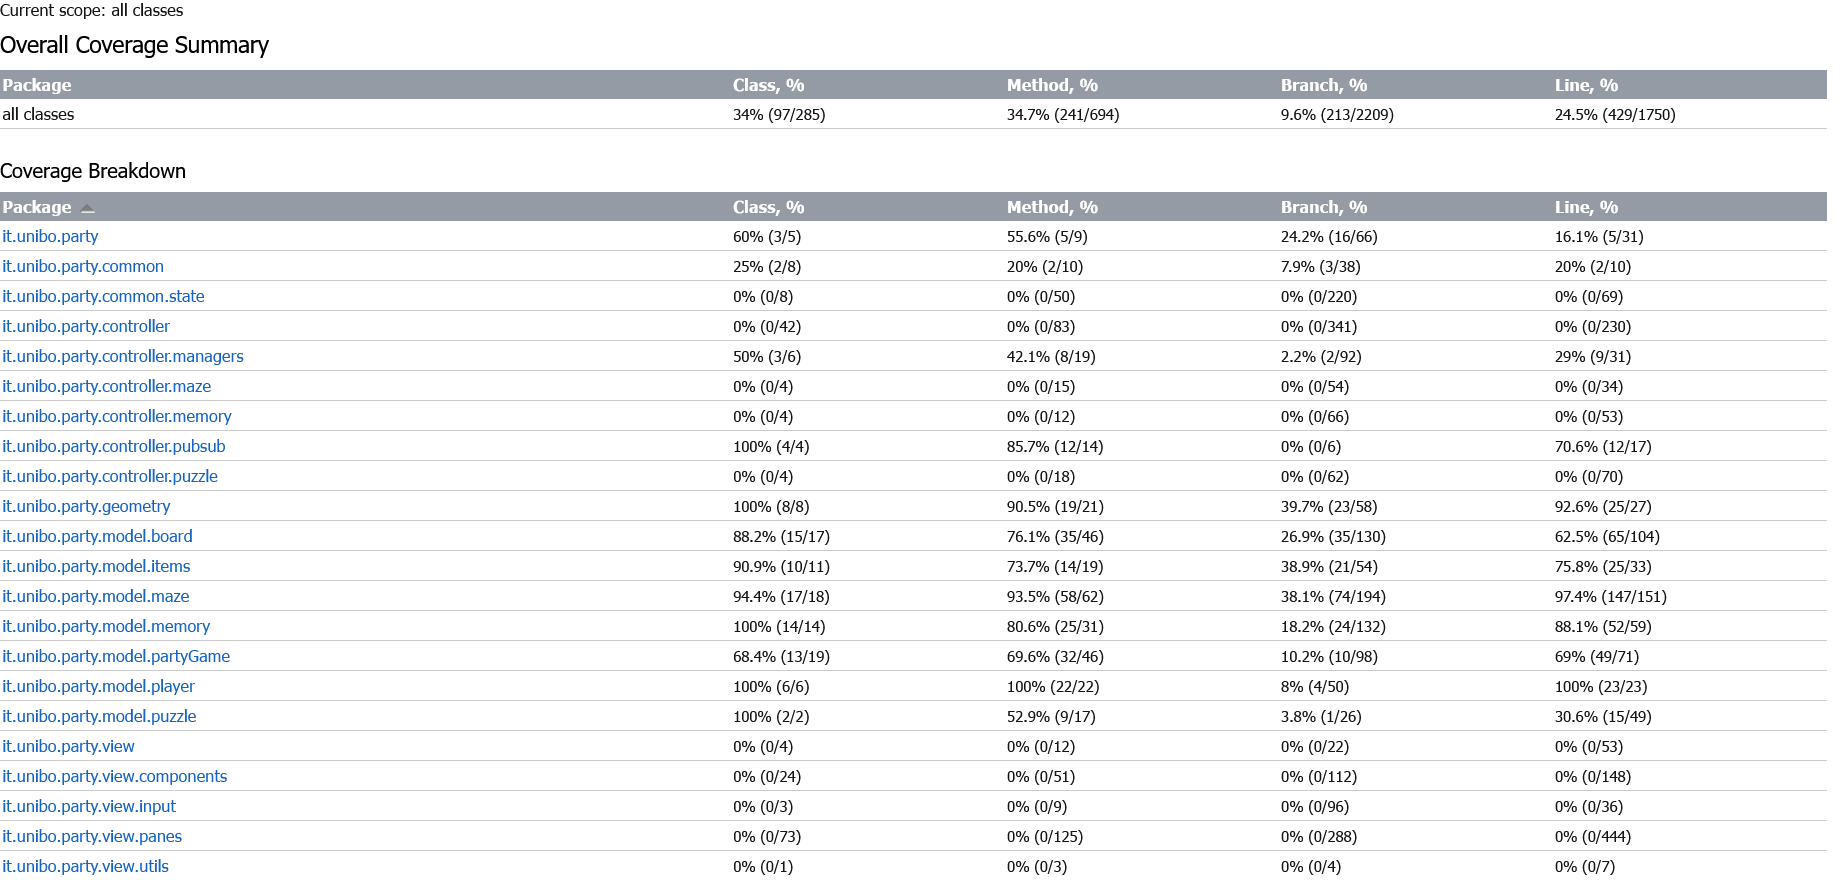
\includegraphics[width=1\textwidth]{figures/testing-coverage.png}
    \caption{Coverage report generato con IntelliJ}
    \label{fig:coverage-report}
\end{figure}

\subsection{Metodologia usata} \label{subsec:testing-methodology}
Come già accennato, il progetto è stato sviluppato utilizzando un approccio TDD (Test Driven Development), quindi i test sono stati
scritti prima della vera implementazione del codice. Come ciclo di TDD abbiamo seguito il ciclo \textit{Red-Green-Refactor} eseguendo
un commit dopo ogni completamento di un ciclo. Solo le classi di model e di utility sono state sviluppate con questo approccio, 
mentre le classi di controller hanno seguito un approccio più classico, scrivendo prima il codice e poi i test.

\subsection{Esempi rilevanti} \label{subsec:testing-examples}
Un esempio rilevante di test è quello del \verb|MazeBuilderTest| che utilizza tecniche di DSL per testare la costruizione di un 
labirinto per il minigioco maze.

\begin{lstlisting}[language=Scala]
    it should "not allow a maze that is not solvable" in:
      val builder: MazeBuilder = MazeBuilder.construct(mazeDimensions._1, mazeDimensions._2):
        W | W | E | W | W
        W | * | * | * | W
        W | * | W | W | W
        W | * | W | W | W
        W | W | X | W | W
      an[IllegalArgumentException] should be thrownBy builder.build()
\end{lstlisting}


\newpage

\section{Restrospettiva}
Durante lo sviluppo di questo progetto il team ha lavorato seguendo un processo
di svuluppo SCRUM-inspired, come consigliato nelle regole del progetto.
In particolare, sono stati effettuati cinque sprint della durata di circa una 
settimana ciascuno. All'inizio e alla fine di ogni sprint il team si è riunito
per discutere i task completati nello sprint precedente e per pianificare i task
dello sprint successivo. È stato utilizzato un foglio di calcolo condiviso per
tenere traccia delle attività tramite un product backlog e degli sprint backlog.
Per ciascuno sprint backlog è stata utilizzata una tabella riempita con le attività 
principali da completare, ciascuna suddivisa in task più piccoli, associati a un
responsabile e a una stima del tempo necessario per il completamento. Durante la settimana 
dedicata allo sprint, sempre tramite lo stesso foglio di calcolo, ciascun membro
del team ha tenuto traccia del tempo realmente impiegato per completare ciascun 
task. Alla fine di ogni sprint la tabella è stata poi inserita nella repository
del progetto come documento di retrospettiva dello sprint.

Questa tipologia di organizzazione si è rivelata molto utile per l'organizzazione
del lavoro e la coordinazione. L'identificazione chiara e continuativa degli obiettivi
da raggiungere ha permesso di ottenere risultati tangibili in tempi brevi e
di avere una visione chiara del progresso del progetto nonché della quantità
di tempo dedicato da ciascun membro del team. 

Di seguito vengono riportati il product backlog (figura \ref{fig:product-backlog}) e gli sprint backlog utilizzati durante lo sviluppo
insieme a un commento sui risultati ottenuti per ciascuno sprint.

\begin{figure}[ht!]
    \centering
    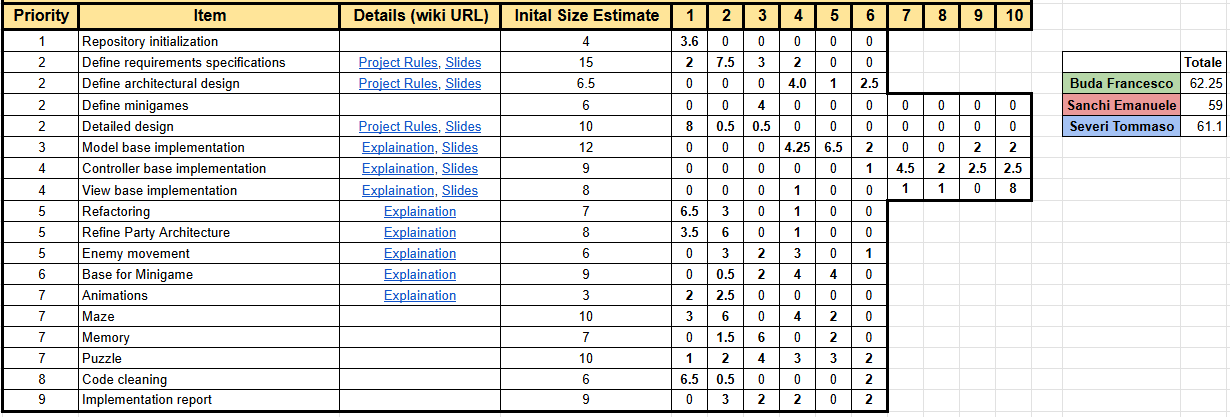
\includegraphics[width=1\textwidth]{figures/product-backlog.png}
    \caption{Product Backlog}
    \label{fig:product-backlog}
\end{figure}

\subsection{Sprint-1} \label{sec:sprint-1}
Il primo sprint (figura \ref{fig:backlog-sprint-1}) è stato dedicato alla definizione dei requisiti
e del design architetturale del progetto, oltre che alla creazione della repository e della struttura 
di base.
\begin{figure}[ht!]
    \centering
    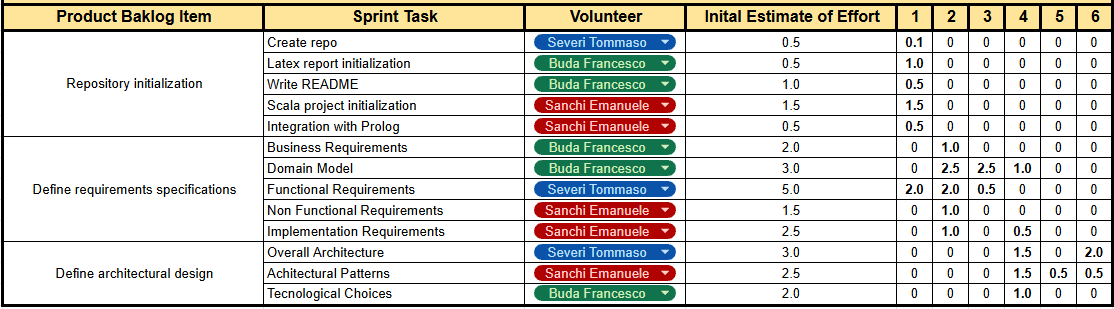
\includegraphics[width=1\textwidth]{figures/backlog-sprint-1.png}
    \caption{Backlog per lo Sprint-1}
    \label{fig:backlog-sprint-1}
\end{figure}
\subsection{Sprint-2} \label{sec:sprint-2}
Il secondo sprint (figura \ref{fig:backlog-sprint-2}) ha portato alla definizione dei minigiochi 
e del design di dettaglio, nonché alla realizzazione di una prima versione funzionante dell'applicazione, 
questa prima versione aveva le seguenti caratteristiche:
\begin{itemize}
    \item Schermata iniziale di Start
    \item Schermata di gioco principale
    \item Movimento del giocatore tramite frecce
    \item Movimento randomico del nemico
    \item Schermata di Game Over
\end{itemize}
\begin{figure}[ht!]
    \centering
    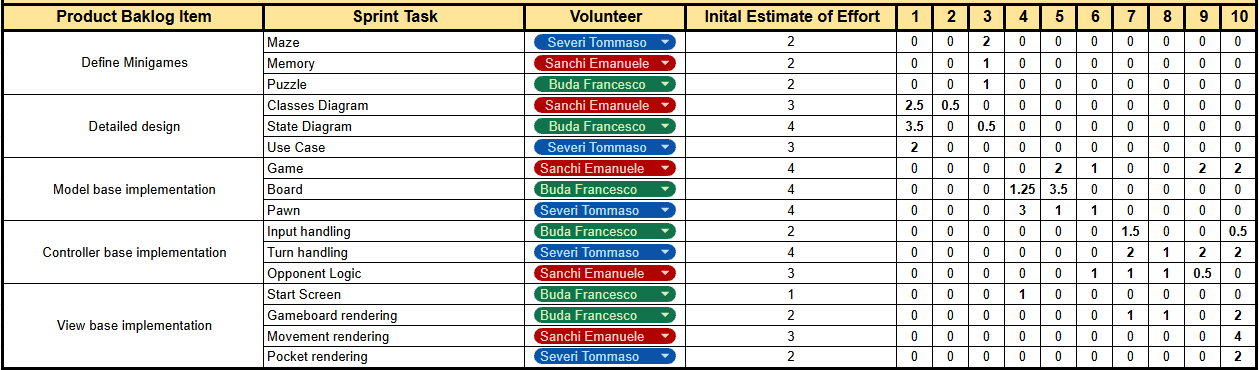
\includegraphics[width=1\textwidth]{figures/backlog-sprint-2.png}
    \caption{Backlog per lo Sprint-2}
    \label{fig:backlog-sprint-2}
\end{figure}
\subsection{Sprint-3} \label{sec:sprint-3}
Il terzo sprint (figura \ref{fig:backlog-sprint-3}) ha segnato il completamento delle funzionalità del
gioco principale e ha posto le basi per l'integrazione dei minigiochi. le funzionalità aggiunte sono state:
\begin{itemize}
    \item tiro di dadi iniziale per decidere il primo giocatore
    \item movimento intelligente del nemico
    \item rigenerazione del tabellone di gioco
    \item doppio tiro di dado per il vincitore di un minigioco
\end{itemize}
\begin{figure}[ht!]
    \centering
    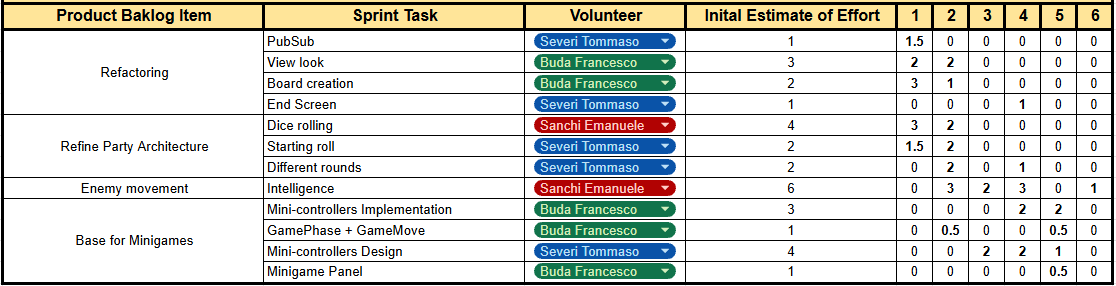
\includegraphics[width=1\textwidth]{figures/backlog-sprint-3.png}
    \caption{Backlog per lo Sprint-3}
    \label{fig:backlog-sprint-3}
\end{figure}
\subsection{Sprint-4} \label{sec:sprint-4}
Il quarto sprint (figura \ref{fig:backlog-sprint-4}) ha aggiunto al gioco principale delle semplici animazioni
e ha completato l'integrazione dei minigiochi maze, memory e puzzle.
\begin{figure}[ht!]
    \centering
    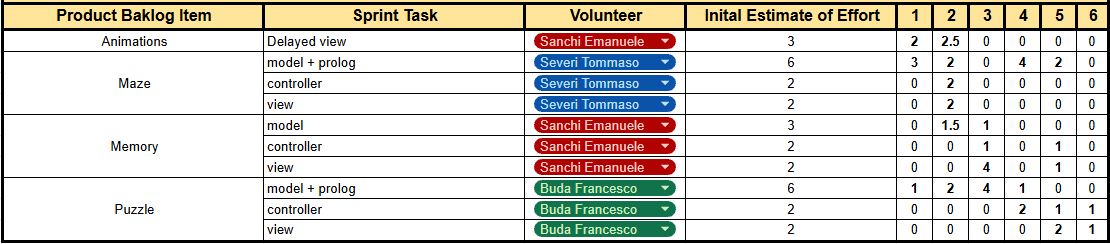
\includegraphics[width=1\textwidth]{figures/backlog-sprint-4.png}
    \caption{Backlog per lo Sprint-4}
    \label{fig:backlog-sprint-4}
\end{figure}
\subsection{Sprint-5} \label{sec:sprint-5}
Lo sprint-5 è stato lo sprint conclusivo del progetto, è stato dedicato alla pulizia del codice e al completamento della documentazione
e della relazione finale.

\begin{figure}[ht!]
    \centering
    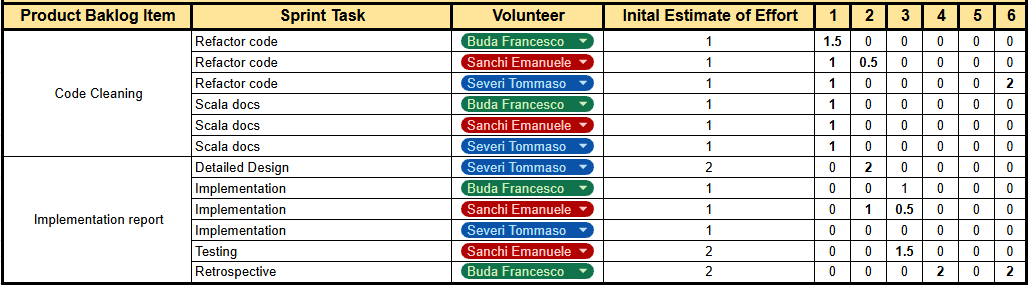
\includegraphics[width=1\textwidth]{figures/backlog-sprint-5.png}
    \caption{Backlog per lo Sprint-5}
    \label{fig:backlog-sprint-5}
\end{figure}
\newpage

\bibliographystyle{plain}
\bibliography{references}

\end{document}